% lista de exercícios 1 - teoria geral de sistemas

\documentclass{article}
\usepackage[a4paper,
            includeheadfoot,
            top=2cm,
            right=2cm,
            bottom=3cm,
            left=3cm]{geometry}
\usepackage[OT1]{fontenc}
\usepackage{parskip}
\usepackage{graphicx}
\usepackage{enumitem}
\usepackage{pifont}
\usepackage{tikz}
\usetikzlibrary{calc, shapes}
\usepackage{amssymb}
\usepackage{amsmath}
\usepackage{hyperref} % cria os links de referencia das equacoes

\begin{document}

\underline{\textbf{Resolução da Lista de Exercícios 1}}\par
\textbf{Sistemas de Informação}\\
\textbf{Instituto Federal do Espírito Santo}\\
Campus Serra\par
\textbf{Teoria Geral de Sistemas}\\
Prof. Dr. Rodrigo Fernandes Calhau\par
Anderson A. Fraga (20222BSI0482)\\
\texttt{aafrg@tuta.io}\\  %\texttt formats the text to a typewriter style font

Dada a \href{http://eprints.rclis.org/20102/1/Kern_Sistemismo_Enancib2011.pdf}{referência}, responda:
\begin{enumerate}
    \item \textbf{Descreva o que cada componente do modelo CESM representa.} \textit{Explique brevemente o significado de Composição, Estrutura, Ambiente e Mecanismo no contexto de um sistema.}
    \item \textbf{Dê um exemplo de um sistema e aplique o modelo CESM para descrevê-lo.} \textit{Escolha um sistema natural, social ou técnico (como uma empresa ou um sistema biológico) e explique sua composição, estrutura, ambiente e mecanismo.}
    \item \textbf{Explique a importância do ambiente em um sistema.} \textit{Usando o modelo CESM, discuta como o ambiente pode influenciar o comportamento de um sistema. Dê exemplos de como o ambiente pode tanto habilitar quanto limitar a função de um sistema.}
    \item \textbf{Diferencie estrutura interna e externa em um sistema conforme o modelo CESM.} \textit{Usando exemplos, explique a diferença entre endoestrutura (ligações internas entre componentes) e exoestrutura (ligações entre o sistema e seu ambiente).}
    \item \textbf{Qual a relação entre a estrutura e o mecanismo de um sistema?} \textit{Explique como que a estrutura de um sistema impacta em seu mecanismo.}
    \item \textbf{Elabore um modelo conceitual sobre o modelo CESM.}
\end{enumerate}\vspace{0.5cm}

Respostas:
\begin{enumerate}
    \item \textit{O modelo CESM é composto por:}\\
        \textbf{Composição}: representa a coleção de partes ou elementos de um sistema;\\
        \textbf{Estrutura}: é a ligação entre componentes e itens que os compõe o sistema;\\
        \textbf{Ambiente}: é a coleção de itens que não fazem parte do sistema, mas atuam ou são influenciados por algum componente dele;\\
        \textbf{Mecanismo}: é o conjunto de processos que, por meio da composição, estrutura e itens ambientais, formam as transformações que causam emergência ou modificação do seu próprio sistema ou de partes dele.
    \item \textit{Em um sistema técnico como um supermercado, pode-se apontar que uma empresa deste ramo é composta por:}\\
        \textbf{Composição}: o corpo de colaboradores juntamente à equipe gerencial e demais atores;\\
        \textbf{Estrutura}: a ligação/relações entre a empresa (conjunto de componentes) e o mercado (relações econômicas entre a empresa e entidades externas);\\
        \textbf{Ambiente}: os regimentos internos visíveis (regras da empresa) e invisíveis (comportamentais, relações de poder entre os componentes, etc.);\\
        \textbf{Mecanismo}: as relações entre colaboradores e clientes que resultam em vendas para o supermercado.
    \item O ambiente é imprescindível para que os sistemas existam, principalmente quando consideramos o ambiente que forma uma empresa de comércio como um supermercado. Sem um ambiente, no caso do modelo CESM escolhido para este exemplo \underline{limitante}, a relação entre produção de um ou mais produtos finais, por meio dos mecanismos disponíveis, se torna difícil e, talvez, até impossível, dada a impossibilidade de troca de informações, de regramento sobre as atividades desenvolvidas e resultados esperados, assim como a falta da avaliação de qualidade sobre o trabalho produzido. Como um exemplo que \underline{habilita} a função do sistema por meio do ambiente é a agilidade na produção de informações e correção de erros produzidos ao longo do processo. O ambiente, neste caso, é o responsável pela viabilização das informações formadas com o andar do comércio de produtos, com a interação entre os componentes, da utilização dos mecanismos necessários para essa interações acontecerem e das tratativas contábeis e de natureza econômicas formadas dentro do ambiente de um supermercado.
    \item A \textbf{estrutura interna} de um supermercado, tomando como base aspectos sociotécnicos deste sistema, representando sua \textit{endoestrutura}, pode ser exemplificada pela relação entre funcionários e a gerência da empresa ou entre funcionários e colaboradores que fornecem os produtos que serão comercializados pelo supermercado, entre outras interações (\textit{estrutura}) entre funcionários (\textit{componentes}) e gerente (\textit{componente}) e colaboradores (\textit{componente}).\\
    Diferente da estrutura interna, restrita a componentes e interações internas à organização, a \textbf{estrutura externa}, ou, neste caso, a \textit{exoestrutura}, é representada pela ligação entre componentes internos a clientes (\textit{componente externo pertencente ao ambiente}), por exemplo, que produzem capital para o supermercado.
    \item A estrtura de um sistema tem grande impacto sobre os mecanismos que atuam sobre ele. De um modo geral, a estrutura é responsável pela forma física em que o mecanismo existe, já que este último não é algo palpável. Então, ao passo em que a estrutura passa a não funcionar de forma correta, os mecanismos e suas cadeias causais também entram na mesma crise, já que ambos são interdependentes.
    \item 
\end{enumerate}
    \begin{figure}[!h]
        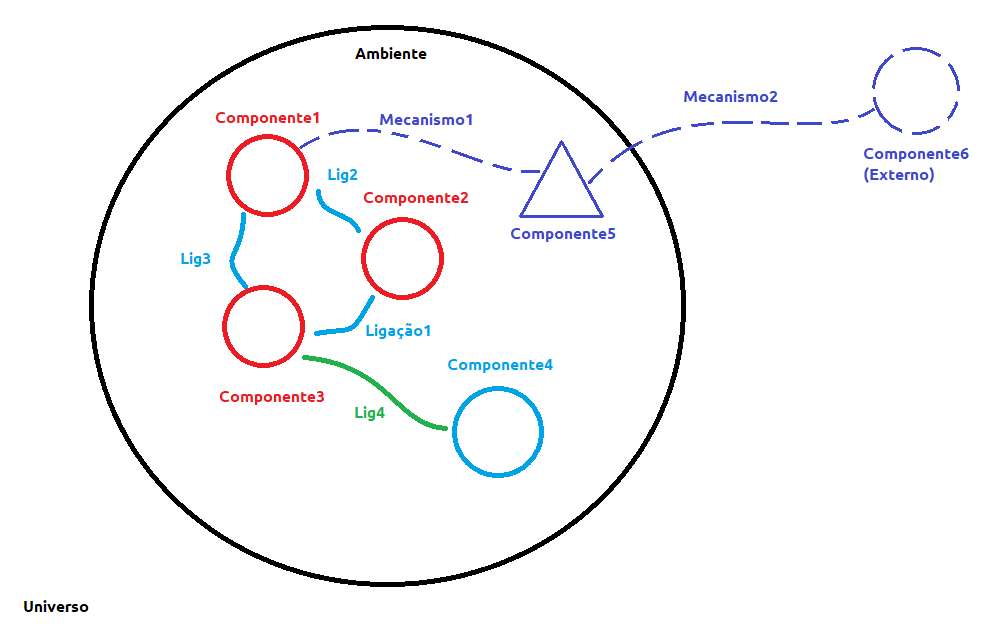
\includegraphics[width=16cm]{modeloConceitualCESM.png}
    \end{figure}
\end{document}